\section{Experimentos numéricos}
\begin{frame}
    \frametitle{Caso para dos niveles}
    \begin{itemize}
        \item Para este ejemplo consideramos el siguiente conjunto de números impares: $\mathcal{E}_a = \{\emptyset\}$ y $\mathcal{E}_b = \{1,5,7,11,13\}$.
        \item Además consideramos el vector objetivo $\bm{b}_T = [m_a,0,0,0,0]$, donde  $m_a \in [0,1]$ es un parámetro.
        \item Compararemos la solución obenida mediante control óptimo con soluciones obtenidas en el problema con número de ángulos prefijados.
        \item Compararemos con las siguientes  penalizaciones: $\mathcal{L}(f) = -f$, $\mathcal{L}(f) = +f$ y $\mathcal{L}(f) = -f^2$
    \end{itemize}
\end{frame}

\begin{frame}
    \frametitle{Caso para dos niveles}
    \begin{figure}
        \centering
        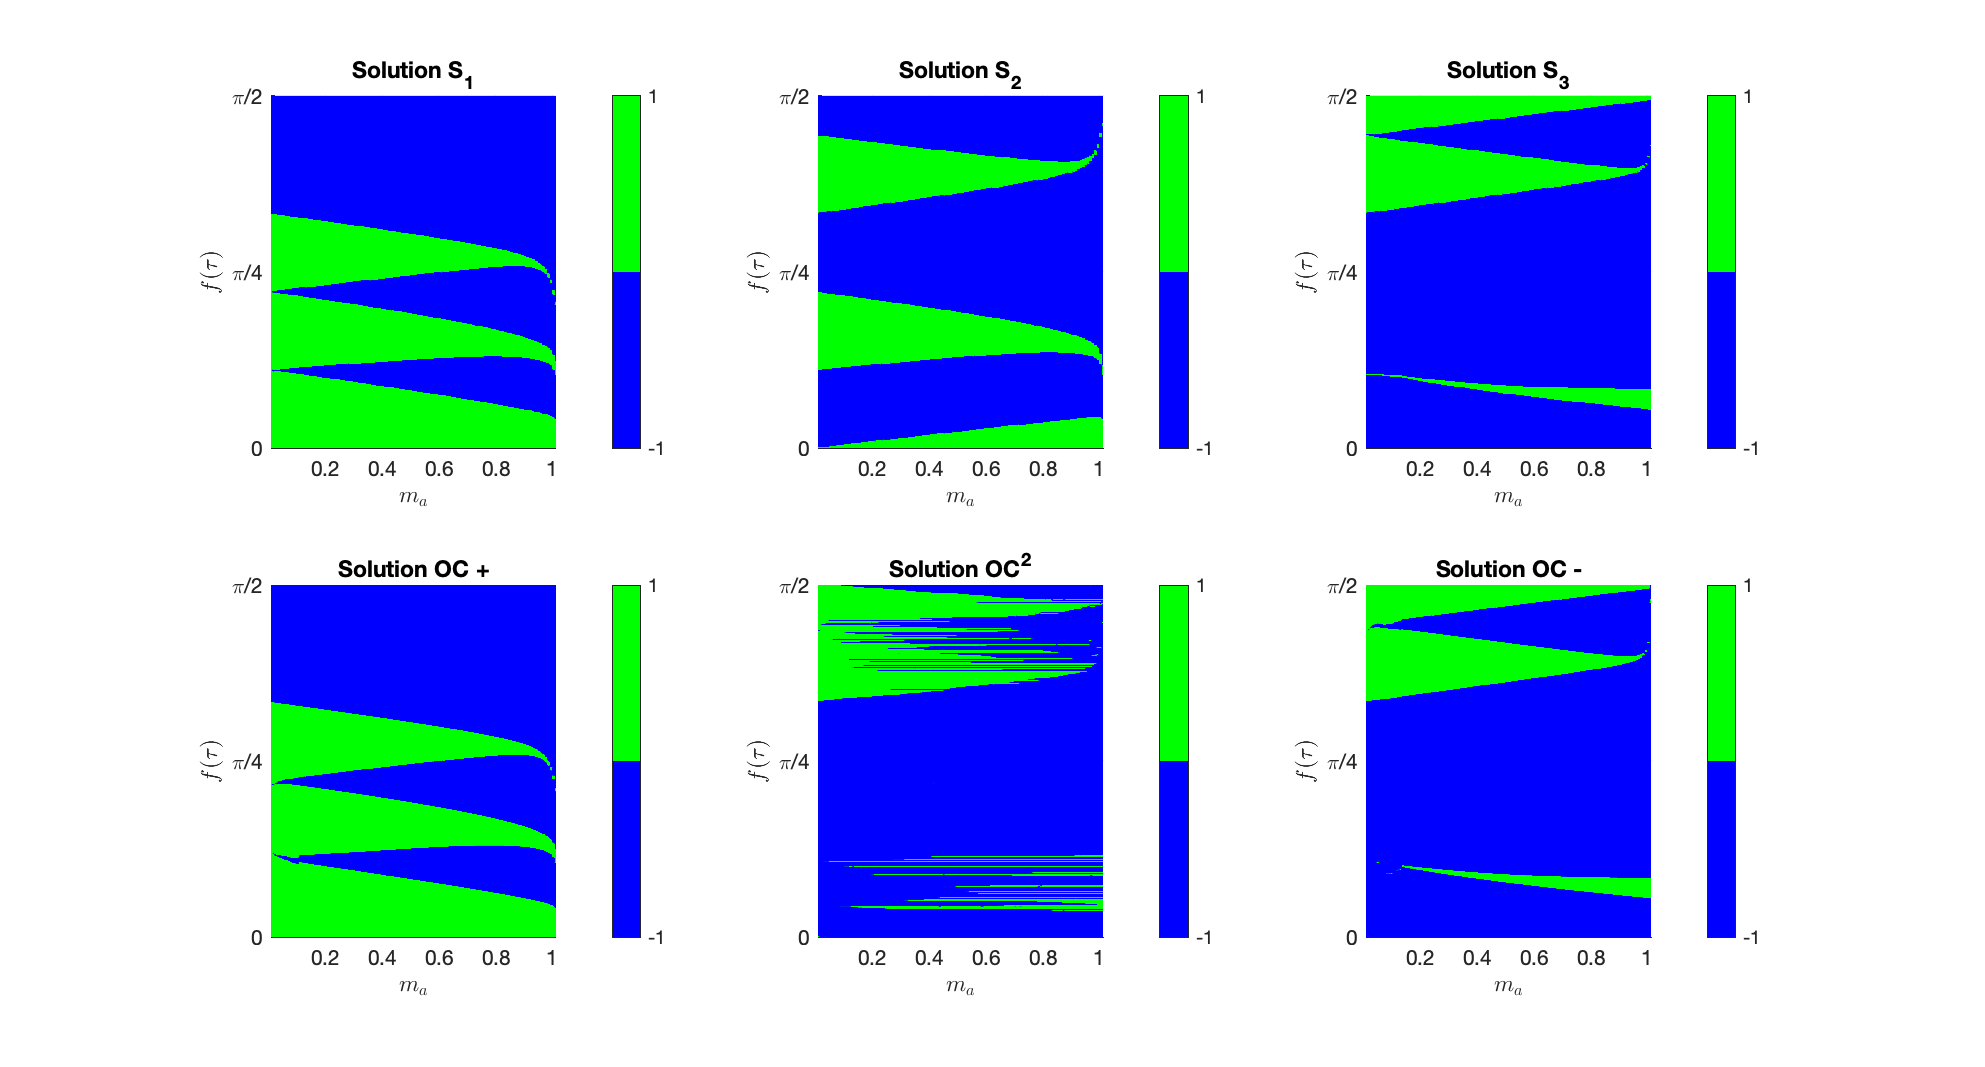
\includegraphics[scale=0.35]{../D0002-FullReport/img/EX01_surf.eps}
    \end{figure}
    
\end{frame}

\begin{frame}
    \frametitle{Caso para tres niveles}
    \begin{itemize}
        \item Podemos ver que en el caso en el que el control $f(\tau)$ solo pueda tomar valores entre $[0,1]$ obtenemos señales que pueden tomar tres niveles en el intervalo $[0,2\pi]$ gracias a la simetría de media de onda.
        \item Si resolvemos el problema de control óptimo pero esta vez cambiando las restricciones $|f(\tau)|<1$ por $\{0<f(\tau)<1\}$.
        \item Se ha realizado el mismo procedimiento que en el caso anterior.
    
    \end{itemize}

\end{frame}
\begin{frame}
    \frametitle{Caso para tres niveles}
    \begin{figure}
        \centering
        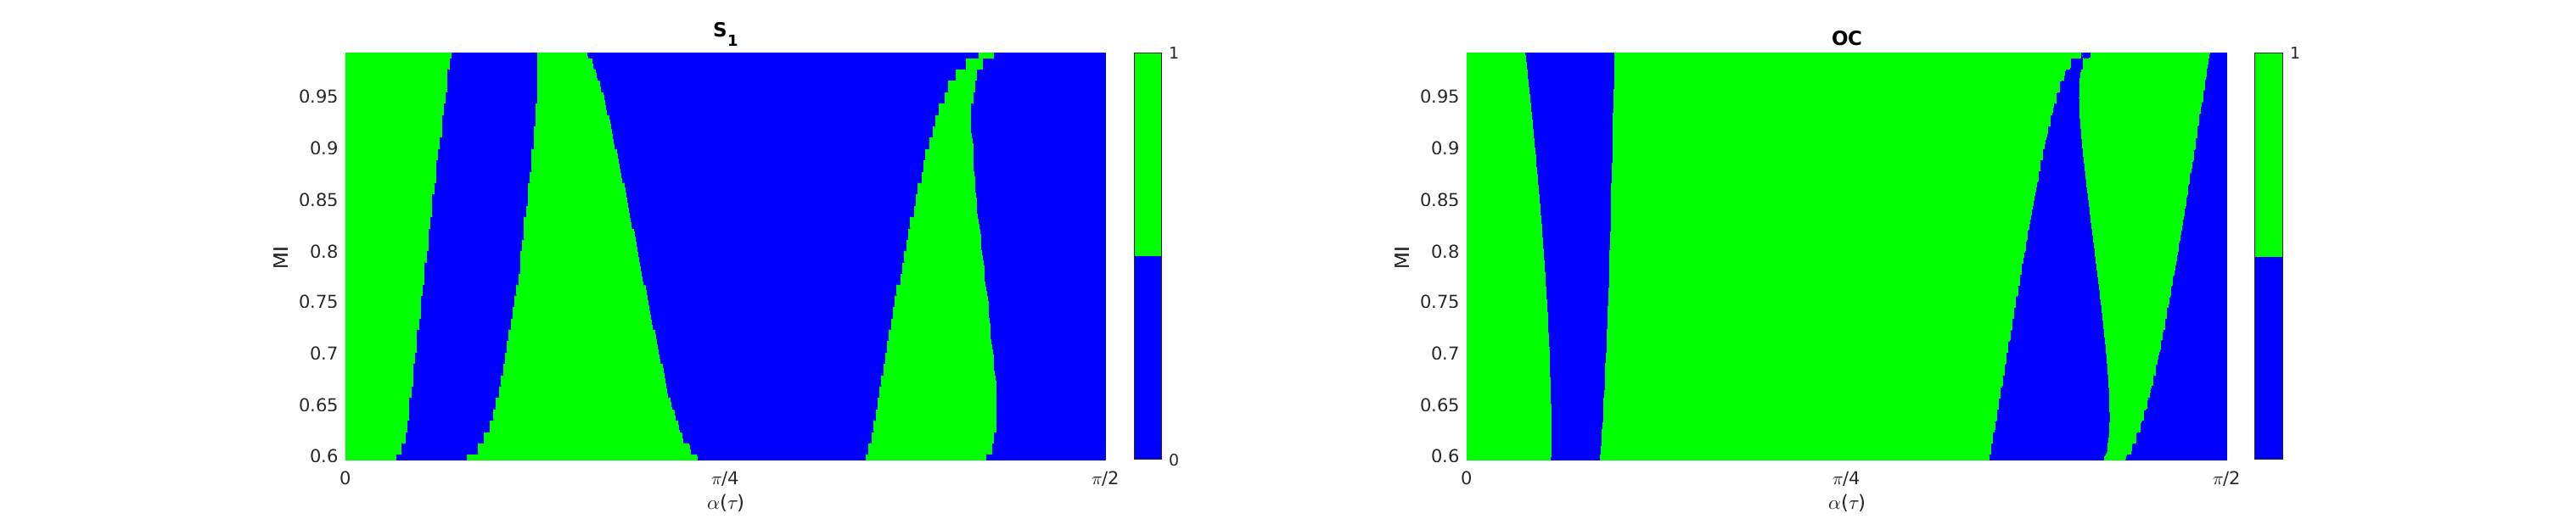
\includegraphics[scale=0.325]{../D0002-FullReport/img/EX01_surf_3LVL.eps}
    \end{figure}
    
\end{frame}
